\question{在均匀外电场中置入半径为\nota{R_0}的导体球,试用分离变量法求出下列两种情况的电势:}

    \subquestion{导体球上接有电池,使球与地保持电势差\nota{\Phi_0};}
        
        \def \P{\Phi_0}
        \def \c{\cos\theta}
        
        一般而言,取地面为电势零点,则球内和球面的电势为\nota{\P}。对于球外空间,为有对称轴的第一类边值问题,其通解为\equa{
            \ph=\sum_n\left( a_nR^n+\frac{b_n}{R^{n+1}} \right)\mathrm{P}_n(\c)
            \quad
            (R>R_0)
            \label{2.1_通解}
        }
        下面考虑边界条件。在无穷远处,表现为匀强场
        \equa{\ph|_{R\to\infty}\to\ph_0-E_0R\c\label{2.1_边界条件1}}
        其中\nota{\ph_0}为任意常数,其物理意义为通过坐标原点的垂直于外场方向的平面在无穷远处的电势。在球面处,由电势连续给出
        \equa{\ph|_{R=R_0}=\P\label{2.1_边界条件2}}
        将(\ref{2.1_通解})分别代入(\ref{2.1_边界条件1})(\ref{2.1_边界条件2}),并由\nota{\{\mathrm{P}_n(\c)\}}的正交完备性,比较系数得到
        \begin{equation}
            \begin{tabular}{llll}
                $a_0 = \ph_0$ \qquad 
                &$a_1 = -E_0$ \qquad 
                &$a_n = 0$ %\quad 
                &$(n\ne0,1)$ \\
                $b_{0} = (\P - \ph_0 )R_0 $ \qquad 
                &$b_1 = -E_0R^3$ \qquad 
                &$b_n = 0 $%\quad 
                &$(n\ne0,1)$
            \end{tabular}
            \label{2.1_系数1}
        \end{equation}
        将(\ref{2.1_系数1})代回(\ref{2.1_通解})得到满足边界条件的特解
        \equa{
            \ph = -E_0R\c + \ph_0 + (\P-\ph_0)R_0\frac{1}{R}+E_0R_0^3\frac{1}{R^2}\c
            \quad
            (R>R_0)
            \label{2.1_特解1}
        }
        
        我们注意到在特解(\ref{2.1_特解1})中,仍有一个未能确定的常数\nota{\ph_0},而非是真正的唯一确定的特解——这是因为我们的边界条件并不是完备的——无穷远处的电势没有well defined。但是,我们需要有所区别的是,这并不意味着无穷远处的电势零点没有确定,电势零点在球面接地时就由地面确定了,这一待定常数其实是和球面上的第二类边界条件球面电荷绑定的。如果在给定球面电势的同时,也给定球面的电荷总量,那么就可以得到唯一确定的通解。这是非常独特的一类边值问题,由于无穷远边界条件的不完备,它需要我们在球面边界上同时给定第一类和第二类边界条件才能得解。
        
        根本而言,这种独特性是源于“不寻常的接地”。在通常情况下,可以取无穷远为电势零点,而接地则意味着电势与无穷远一致为零,这样就能确定有限边界和无穷远边界的电势差值(我们知道,电势的差值才有物理意义),从而得到有物理意义的解。而在本题情形,由于无穷远处存在匀强电场,无穷远的电势不是唯一的,无法取无穷远为电势零点,这样以来,“接地”就失去了它真正有物理意义之处,无法给定边界与边界的电势差值,而只是在形式上给了一个电势零点。严谨地讲,这种无穷远处仍存在电场的情形甚至不能用接地来定义电势零点,因为这种情况下所谓的“地”里面也该是存在电流的,故而“地”的电势也不唯一了。
        
        当然,如果只是就题做题,从数学上来讲,我们还是能在形式上给出(\ref{2.1_特解1})这样一个不完备的通解的,这并没有什么问题。
    
    \subquestion{导体球上带有总电荷\nota{Q};}
    
        这种情况下仍然可以沿用(\ref{2.1_通解})和(\ref{2.1_边界条件1})。而(\ref{2.1_边界条件2})则需要改写为第二类边界条件,由高斯定理与静电场的边值关系得
        \equa{
            -\eps_0\int\limits_{R=R_0}\frac{\partial \ph}{\partial R}R^2\d \Omega = Q
            \label{2.1_边界条件3}
        }
        将通解(\ref{2.1_通解})代入边界条件(\ref{2.1_边界条件1})(\ref{2.1_边界条件3}),并由\nota{\{\mathrm{P}_n(\c)\}}的正交完备性,比较系数得到
        \begin{equation}
            \begin{tabular}{llll}
                $a_0 = \ph_0$ \qquad 
                &$a_1 = -E_0$ \qquad 
                &$a_n = 0$ %\quad 
                &$(n\ne0,1)$ \\
                $b_{0} = \frac{Q}{4\pi\eps_0} $ \qquad 
                &$b_1 = -E_0R^3$ \qquad 
                &$b_n = 0 $%\quad 
                &$(n\ne0,1)$
            \end{tabular}
            \label{2.1_系数2}
        \end{equation}
        将(\ref{2.1_系数2})代回通解(\ref{2.1_通解})得到满足边界条件的特解
        \equa{
            \ph = -E_0R\c + \ph_0 + \frac{Q}{4\pi\eps_0}\frac{1}{R}+E_0R_0^3\frac{1}{R^2}\c
            \quad
            (R>R_0)
            \label{2.1_特解2}
        }
        
        这里的特解(\ref{2.1_特解2})仍然只能确定至相差一个任意常数\nota{\ph_0},它出现的理由和之类的论述是一致的,仍然是由于(\ref{2.1_边界条件1})的不完备性所致,或者这里也可以简单理解为电势零点的不确定性。\nota{\ph_0}和球面的电势是绑定的,如果我们同时再给球面加一个第一类边界条件,确定球面的电势,那么这一\nota{\ph_0}也就可以唯一确定了。
        
    \subquestion{(讨论)导体球上接有电池,使球与地保持电势差\nota{\Phi_0};\textbf{同时}导体球上带有总电荷\nota{Q}.}
        
        那么综上所述,如果在球面同时给定两类边界条件(在无穷远边界不完备的情况下),即给定球面电势\nota{\P}和总电荷\nota{Q},则可以确定唯一的特解。我们联立(\ref{2.1_通解})(\ref{2.1_边界条件1})(\ref{2.1_边界条件2})和(\ref{2.1_边界条件3}),解得,或者直接比较(\ref{2.1_特解1})(\ref{2.1_特解2})得到
        \equa{
            \ph = -E_0R\c + \P + \frac{Q}{4\pi\eps_0}(\frac{1}{R}-\frac{1}{R_0})+E_0R_0^3\frac{1}{R^2}\c
            \quad
            (R>R_0)
            \label{2.1_特解3}
        }
        此即在球面同时满足完备的两类边界条件的唯一确定的特解。

\question{在接地的导体平面上有一半径为\nota{a}的半球凸部(如图),半球的球心在导体平面上,点电荷\nota{Q}位于系统的对称轴上,并与平面相距为\nota{b(b>a)},试用电像法求空间电势.}

    \begin{figure}[htbp]
        \centering
        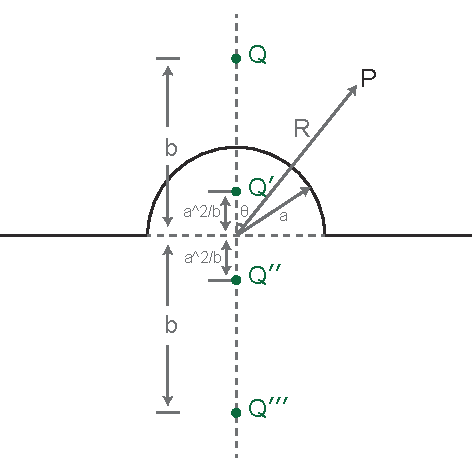
\includegraphics[width=10cm]{img/2.1/电像法1.pdf}
        \caption{导体平面上的半球}
        \label{2.1_fig:电像法1}
    \end{figure}
    
    如图\ref{2.1_fig:电像法1}放置三个镜像电荷\nota{Q'}、\nota{Q''}、\nota{Q'''}。它们的带电荷量分别为
    \begin{eqnarray}
        Q'   &=& -\frac{a}{b}Q \\
        Q''  &=& +\frac{a}{b}Q \\
        Q''' &=& -Q
    \end{eqnarray}
    这一的镜像电荷放置方案是由我们熟知的接地无穷大导体平面、接地导体球的镜像方案组合而成。容易看出,对于球面电势为0条件而言,\nota{Q}和\nota{Q'}作为一对镜像电荷使球面使球面等势为0,\nota{Q''}和\nota{Q'''}作为一对镜像电荷使球面等势为0,则它们的叠加当然也满足球面等势为0;对于导体平面电势为0条件而言,\nota{Q}和\nota{Q'''}作为一对镜像电荷使导体平面电势为0,\nota{Q'}和\nota{Q''}作为一对镜像电荷使导体平面电势为0,则它们的叠加当然也满足导体平面电势为0。
    
    这一以来,由静电场的唯一性定理可知,有如下唯一的电势解
    \begin{multline}
        \ph(R,\theta,\phi) = \frac{Q}{4\pi\eps_0 R}
        \left[
            \frac{+1}{\sqrt{1+\left(\frac{b}{R}\right)^2-2\left(\frac{b}{R}\right)\c}}
            +\frac{-1}{\sqrt{1+\left(\frac{b}{R}\right)^2+2\left(\frac{b}{R}\right)\c}}
            \right.
            \\
            \left.
            +\frac{-a/b}{\sqrt{1+\left(\frac{a^2}{bR}\right)^2-2\left(\frac{a^2}{bR}\right)\c}}
            +\frac{+a/b}{\sqrt{1+\left(\frac{a^2}{bR}\right)^2+2\left(\frac{a^2}{bR}\right)\c}}
        \right]
        \quad(R>a,0\le\theta<\pit)
    \end{multline}
    当然也容易验证,当\nota{R=a}或\nota{\theta=\pit}时,\nota{\ph(R,\theta,\phi)\equiv 0}。
    
    对于导体平面及其下方的区域,由于静电屏蔽,有
    \equa{
        \ph(R,\theta,\phi)\equiv 0 \quad(0\le R\le a\cup\pit\le\theta\le\pi)
    }

\question{有一点电荷\nota{Q}位于两个相互垂直的接地导体平面所围成的直角空间内,它到两个平面的距离为\nota{a}和\nota{b},求空间电势.}

    \begin{figure}[htbp]
        \centering
        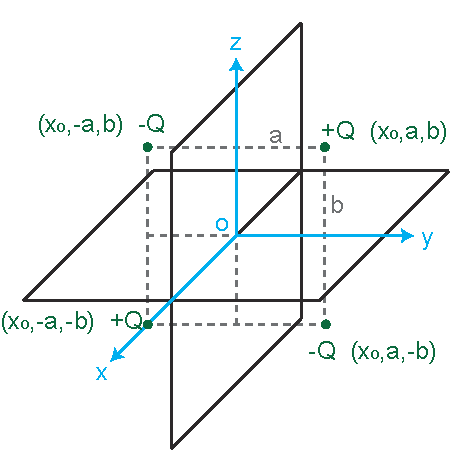
\includegraphics[width=10cm]{img/2.1/电像法2.pdf}
        \caption{两个垂直的导体平面}
        \label{2.1_fig:电像法2}
    \end{figure}
    
    如图\ref{2.1_fig:电像法2}放置三个镜像电荷,电荷量和坐标都已标示在图中。这一镜像电荷放置方案使根据单个无穷大接地 导体平面模型组合而来的,镜像电荷两两使得导体平面电势为零。
    
    由静电场的唯一性定理可知,有如下唯一的电势解
    \begin{multline}
        \ph(R,\theta,\phi)=\\
        \left\{
        \begin{aligned}
        	&\frac{Q}{4\pi\eps_0}
        	\left[ 
        	    \frac{+1}{\sqrt{(x-x_0)^2+(y-a)^2+(z-b)^2}}
        	    +\frac{-1}{\sqrt{(x-x_0)^2+(y+a)^2+(z-b)^2}}\right.&  \\
        	    &\left.+\frac{-1}{\sqrt{(x-x_0)^2+(y-a)^2+(z+b)^2}}
        	    +\frac{+1}{\sqrt{(x-x_0)^2+(y+a)^2+(z+b)^2}}
        	\right],
        	&(y>0,z>0)\\
        	& \qquad\qquad\qquad\qquad\qquad\qquad\qquad\qquad 0, &
        	\mathrm{else}
    	\end{aligned}
        \right.
    \end{multline}
    

\question{(附加题)一半径为\nota{R_0}的球面,在球坐标\nota{0<\theta<\frac{\pi}{2}}的半球面上电势为\nota{\ph_0},在\nota{\frac{\pi}{2}<\theta<\pi}的半球面上电势为\nota{-\ph_0},求空间各点电势.}

    \def \g{G(R,\theta,\phi;R',\theta',\phi')}
    \def \gr{Green函数}

    本题为第一类边值问题,定义Green函数为
    \equa{
        \nabla^2\g=-\frac{1}{\eps_0}\delta(R-R',\theta-\theta',\phi-\phi')
        \quad (0<R<R_0\cup R>R_0) \label{2.1_格林函数定义1}
    }
    \equa{
        \g|_{R=R_0}=0 \label{2.1_格林函数定义2}
    }
    原则上来讲,球内球外的\gr{}需要分别定义,因为它们是两个独立的求解区域。这里只是简便地将它们写成同一个格林函数,毕竟它们的解恰好在形式上是相同的,为
    \begin{multline}
        \g =\\ \frac{1}{4\pi\eps_0}
        \left[
            \frac{1}{\sqrt{R^2+R^2-2RR'\cos(\theta-\theta')}}
            -\frac{1}{\sqrt{\left(\frac{RR'}{R_0}\right)^2+R_0^2-2RR'\cos(\theta-\theta')}}
        \right]\label{2.1_格林函数的解}
    \end{multline}
    并且该解中的\nota{R,\theta,\phi}和\nota{R',\theta',\phi'}在形式上是对称的,因此可以将
    \equa{G(R',\theta',\phi';R,\theta,\phi)=\g=G}
    都简记为\nota{G}。
    
    在球内和球外无自由电荷,即
    \equa{\rho(R',\theta',\phi')=0} \label{2.1_自由电荷}
    根据Green formula得到电势解的形式
    \equa{
        \ph(R,\theta,\phi)=\eps_0\int\limits_{R'=R_0}\ph(R',\theta',\phi')
        \frac{\partial}{\partial n}G(R',\theta',\phi';R,\theta,\phi)\d S' \label{2.1_格林公式}
    }
    其中已代入(\ref{2.1_格林函数定义2})(\ref{2.1_自由电荷})来化简。
    
    球内和球外关于球面法向\nota{n}的定义是不同的,由此(\ref{2.1_格林公式})具体写为
    \begin{multline}
        \ph(R,\theta,\phi)=\\
        \left\{
        \begin{aligned}
        	&-2\pi\eps_0 R_0^2
        	\left[  
        	    \int_0^{\pit}\ph_0\left.\frac{\partial G}{\partial R'}\right|_{R'=R_0}\sin\theta\d\theta\right. & \\
        	    &\left.\qquad\qquad\qquad + \int_\pit^{\pi}\left(-\ph_0\right)\left.\frac{\partial G}{\partial R'}\right|_{R'=R_0}\sin\theta\d\theta
        	\right] 
        	&\left(R>R_0\right)& \\
        	&-2\pi\eps_0 R_0^2
        	\left[  
        	    \int_0^{\pit}\ph_0\left(-\left.\frac{\partial G}{\partial R'}\right|_{R'=R_0}\right)\sin\theta\d\theta\right. & \\
        	    &\left.\qquad\qquad\qquad + \int_\pit^{\pi}\left(-\ph_0\right)\left(-\left.\frac{\partial G}{\partial R'}\right|_{R'=R_0}\right)\sin\theta\d\theta
        	\right] 
        	&\left(0<R<R_0\right)& 
    	\end{aligned}
        \right.\label{2.1_电势解}
    \end{multline}
    其中
    \equa{
        \left.\frac{\partial G}{\partial R'}\right|_{R'=R_0}=\frac{1}{4\pi\eps_0 R_0^2}\frac{r^2-1}{\left[1+r^2-2r\cos(\theta-\theta')\right]^{\frac{3}{2}}}\label{2.1_8}
    }
    并已简记
    \equa{r=\frac{R}{R_0}>0}\label{2.1_9}
    % \equa{z_0=\cos\theta}\label{2.1_10}
    
    将(\ref{2.1_8})(\ref{2.1_9})代入(\ref{2.1_电势解})得
    \begin{equation}
        \ph(R,\theta,\phi)=
        \left\{
        \begin{aligned}
        	&-\frac{\ph_0}{2}
        	\left(\int_0^{\pit}-\int_{\pit}^{\pi}\right)
        	\frac{r^2-1}{\left[1+r^2-2r\cos(\theta-\theta')\right]^{\frac{3}{2}}}\sin\theta'\d\theta'
        	&r>1 \\
        	&\frac{\ph_0}{2}
        	\left(\int_0^{\pit}-\int_{\pit}^{\pi}\right)
        	\frac{r^2-1}{\left[1+r^2-2r\cos(\theta-\theta')\right]^{\frac{3}{2}}}\sin\theta'\d\theta'
        	&r<1
    	\end{aligned}
        \right.
    \end{equation}
    将源点最后的自由度\nota{\theta'}积掉,就可以(再不济也能在数值层面)得到电势\nota{\ph(R,\theta,\phi)}的表达式。该过程涉及第二类椭圆积分,我就不给出结果了。
    
    有趣的是,我们发现球内和球外的电势在形式上只相差一个负号。我们可以把它们统一写为
    \begin{equation}
        \ph(R,\theta,\phi)=
    	-\frac{\ph_0}{2}
    	\left(\int_0^{\pit}-\int_{\pit}^{\pi}\right)
    	\frac{\left|r^2-1\right|}{\left[1+r^2-2r\cos(\theta-\theta')\right]^{\frac{3}{2}}}\sin\theta'\d\theta'
    \end{equation}
